\newpage

\section{Vorgehen}

TODO: In Anhang verschieben?

Es wurde beschlossen, nach SODA \cite{HSLU-Education-SODA} vorzugehen.
SODA ist eine einfache und agile Vorgehensweise zur Entwicklung von (Software-)Projekten. Dieses Vorgehensmodell wurde von der Hochschule Luzern entwickelt, um den Studenten eine iterativ/inkrementelle Vorgehensweise zu bieten, welche trotzdem zeitlich begrenzt ist. Somit ist es eine Mischung aus dem Wasserfallmodell und Scrum. Scrum wird häufig in der Software Entwicklung eingesetzt, wurde aber ursprünglich aus Studien von Manufakturen wie der Autoindustrie entwickelt \cite{Wikipedia-Scrum-History}.

Da es sich in \acrshort{pren2} nicht um ein reines Software-, sondern um
ein Interdisziplinäres Projekt handelt, besteht die Gefahr, dass Aufgaben
mit niedrigerer Priorität nicht umgesetzt werden. Aus diesem Grund ist es
wichtig, bereits im Vorhinein mögliche Risiken zu identifizieren und deren Machbarkeit
abzuklären. Dies wurde mittels \nameref{sec:design-thinking} gemacht.

Um zu vermeiden dass niedriger priorisierte Aufgaben nicht vernachlässigt werden,
ist es wichtig ein gutes Backlogmanagement zu erstellen. Das heisst alle Aufgaben/Stories zu definieren (siehe \ref{tab:anforderungsliste}), zu schätzen und zu priorisieren. Damit kann bereits früh festgestellt werden, welche Aufgaben zeitlich umgesetzt werden können.

Es werden wöchentliche Stand-Ups mit dem Coach und allen Teammitgliedern durchgeführt, hierbei wird besprochen, was in der letzten Woche erreicht wurde, was für Risiken und Hindernisse bestehen (siehe \nameref{sec:risikomanagement}) und was bis zum nächsten Stand-Up erreicht werden soll.

Als Scrum-Board wird Trello\footnote{https://trello.com/} verwendet.

\newpage

\subsection{Organigramm}
SODA gibt die folgenden Rollen vor:

\begin{items}
  \item {\bf \acrfull{po}} \\
    Repräsentiert die Kunden des Produktes gegenüber dem Team 
    und ist verantwortlich um einen Business-Value zu generieren.
  \item {\bf \acrfull{sm}} \\
    Entfernt Hindernisse, die das Team an der Producktentwicklung hindern.
  \item {\bf Entwicklungsteam} \\
    Ist für die Entwicklung des Producktes zuständig.
\end{items}

Die Rollen wurden gemäss dem Organigramm in Abbildung \ref{fig:organigramm} auf das Team verteilt. Natürlich sind im Rahmen der \acrshort{pren1} Arbeit alle Teammitglieder teil des Entwicklerteams.
Je nach Rolle kann aber mehr oder weniger Arbeit beispielsweise für das Backlogmanagement anfallen.

\begin{figure}[H]
  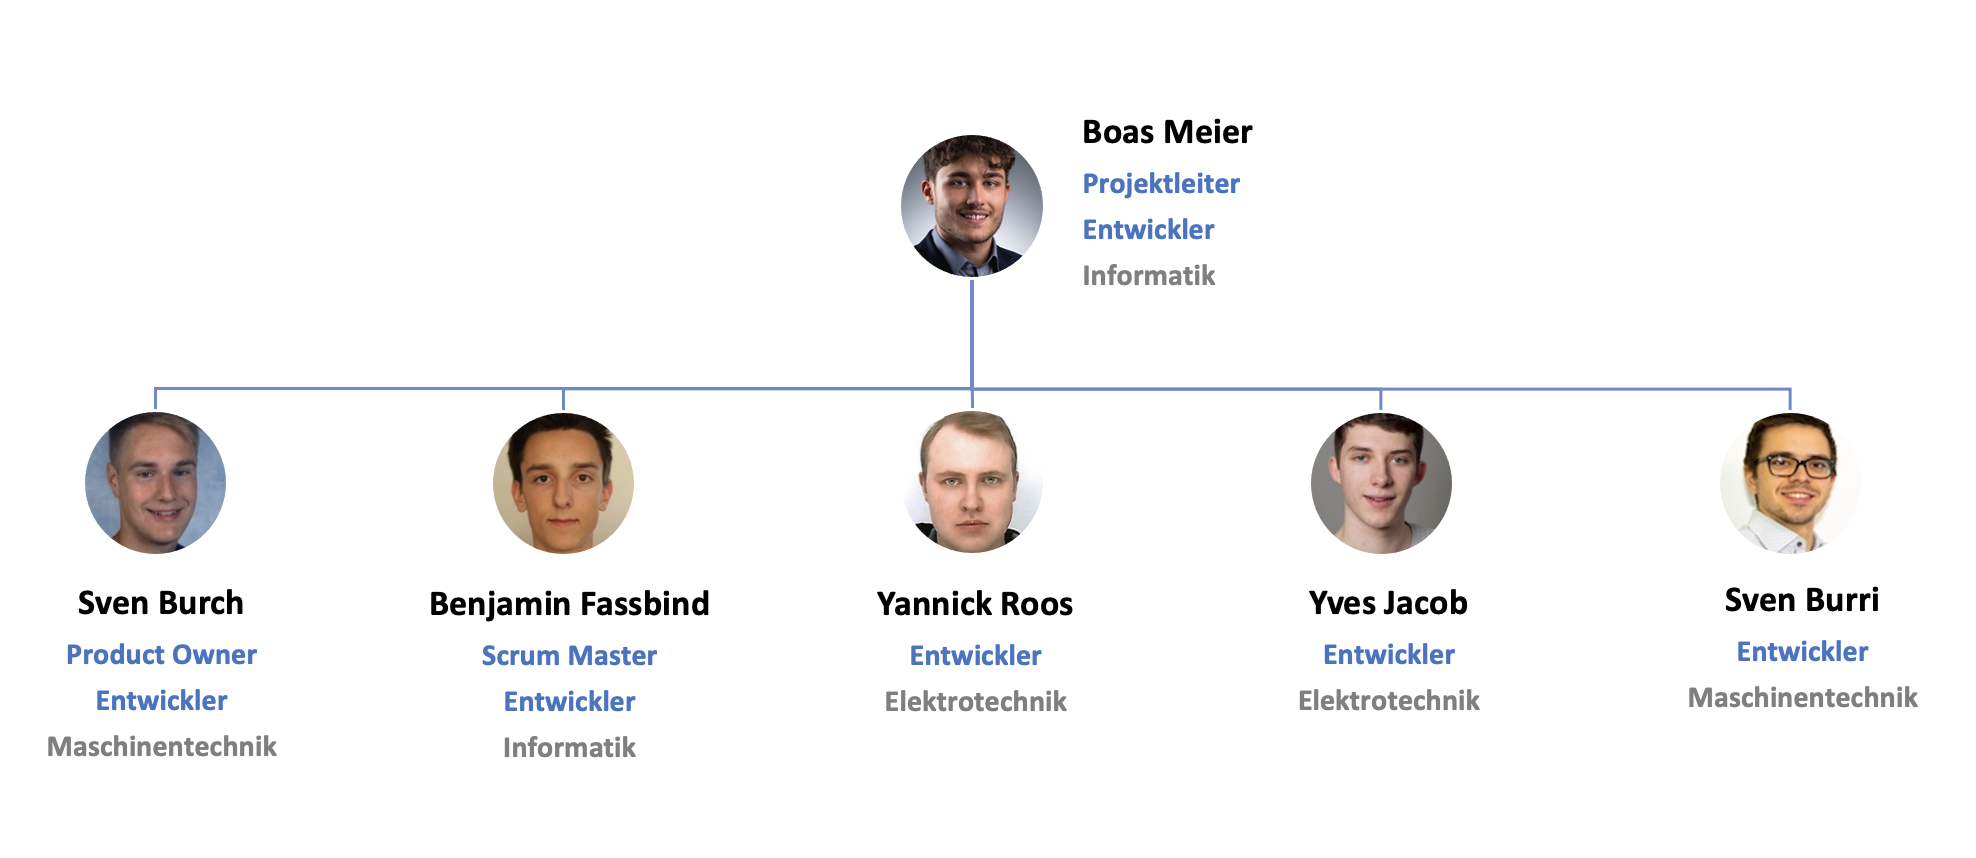
\includegraphics[width=1.0\textwidth]{img/projektmanagement/Organigramm PREN2.png}
  \centering
  \caption{Organigramm Team 05}
  \label{fig:organigramm}
\end{figure}

\newpage

\subsection{Datenaustausch}
Um Daten im Team auszutauschen und gemeinsam Dokumente zu erarbeiten, werden zwei verschiedene Cloud Plattformen verwendet. Jedes Teammitglied hat vollständigen Zugriff auf beide Plattformen.\\

\textbf{OneDrive}\\
Microsoft OneDrive wird verwendet, um Office 365 Dokumente zu verwalten. Dank OneDrive sind diese Dokumente versionskontrolliert und unter allen Mitgliederen synchronisiert. Dies erlaubt eine simultane Bearbeitung.\\

\textbf{GitHub}\\
Mit Hilfe von GitHub wird der Quellcode versionskontrolliert verwaltet. Es wurden zwei Repositories angelegt. Die \LaTeX-Dokumentation ist unter dem Repository https://github.com/randombenj/hslu-pren1-doc erreichbar und der Quellcode unter https://github.com/randombenj/hslu-pren1.

\newpage

\subsection{Design Thinking}
\label{sec:design-thinking}


Bei Design Thinking \cite{Wikipedia-Design-Thinking} geht es in erster Linie darum, strukturiert 
Ideen für die Umsetzung eines neuen Produktes zu finden. Auch soll das Design Thinking
dabei helfen, zu sehen, ob eine Idee umsetzbar ist. Dies wird dadurch erreicht,
dass sehr einfache (\acrshort{lofi}) Prototypen, beispielsweise aus Karton, 
gefertigt werden, um zu sehen, ob das gewünschte Konzept überhaupt umsetzbar ist.

Ein Ansatz des Design Thinking ist der Double Diamond Prozess. Auch dabei geht es
darum, dass man mit einem Problem konfrontiert wird, im hier dargelegten Fall durch die 
Aufgabenstellung, und versucht dabei die bestmögliche Lösung zu finden.

Die Idee dabei ist relativ einfach: Man unterteilt die Problemlösung in vier Teile.
Als erstes versucht man, möglichst breit gefächert das Problem zu verstehen. Dies geschieht
beispielsweise indem man sich mit den Kunden zusammensetzt und sich mit ihnen über das Problem unterhält.
Danach definiert man eine konkrete Problemstellung auf die man sich fokussiert.
In einer dritten Phase versucht man breit gefächerte Ideen zur Lösung des Problems zu finden.
Diese Ideen können auch durchaus unkonventionell sein, es sollte noch nichts ausgeschlossen werden.
Als nächstes definiert man aus den gefundenen Ideen
die besten, welche sich aufgrund von gewissen Kriterien für die Lösung eignen.
Diese klärt man mithilfe von Prototypen auf die Machbarkeit.
\begin{figure}[H]
  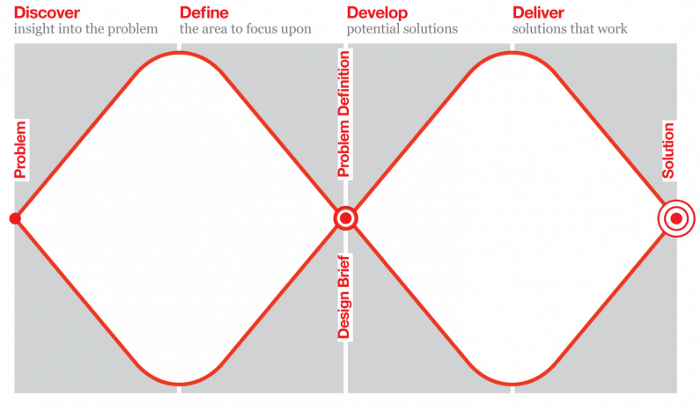
\includegraphics[width=1.0\textwidth]{img/Aufgabenstellung/double-diamond.png}
  \centering
  \caption{Design Thinking mithilfe von Double Diamond}
\end{figure}
  
\subsection{Risikomanagement}
\label{sec:risikomanagement}

Das Risikomanagement wird iterativ-inkrementell jede Woche in den Stand-Ups durchgeführt. Dazu wurde ein Excel-Template verwendet, welche als Datei dem Anhang beigelegt wird. In diesem Template wurde jedem Risiko einen Risk Score zugeteilt, welcher sich aus Eintrittshäufigkeit multipliziert mit Schadensausmass errechnet. Anhand dieses Risk Scores wurde eine Risikomatrix erstellt, welche in Abbildung \ref{fig:risk-matrix} ersichtlich ist. Dieser Risk Score wurde vor und nach der definierten Prävention berechnet (siehe Abbildung \ref{fig:risk-matrix-after-measures}). Nachfolgend in der Tabelle \ref{tab:risikomanagement} werden lediglich die wichtigsten technischen Risiken und deren präventiven Massnahmen aufgelistet. 

\begin{center}
\begin{table}[H]
    \begin{tabularx}{\textwidth}{|l|X|X|}
        \hline
        \textbf{ID} & \textbf{Titel} & \textbf{Vorbeugende Massnahmen} \\ \hline
        R1 & Drehung in der Nähe der Treppenwand. & Stellung der Ausleger so einstellen, dass diese nicht mehr anschalgen können. \\ \hline
        R2 & Gleichgewicht bei Erklimmung & Hebemechanismus im ersten Sprint testen. \\ \hline
        R3 & Roboter verschiebt Hindernisse & Bereits frühe Tests mit ausgesuchter Implementation des CNN. \\ \hline 
        R4 & Technische Limitation Neural Network & Ausgiebige Recherche und Tests bezüglich Performance im Sprint 1 und 2.\\ \hline
        R5 & Unbekannte Position der Ausleger & Ausgiebige Tests im Sprint 1 und 2 um die Schwere des Problems genauer einschätzen zu können. \\ \hline
    \end{tabularx}
    \caption{Risikomanagement}
    \label{tab:risikomanagement}
\end{table}
\end{center}

TODO: Risikomatrizen sind noch nicht aktuell!

\begin{figure}[H]
  \centering
  \begin{minipage}[t]{0.45\linewidth}
  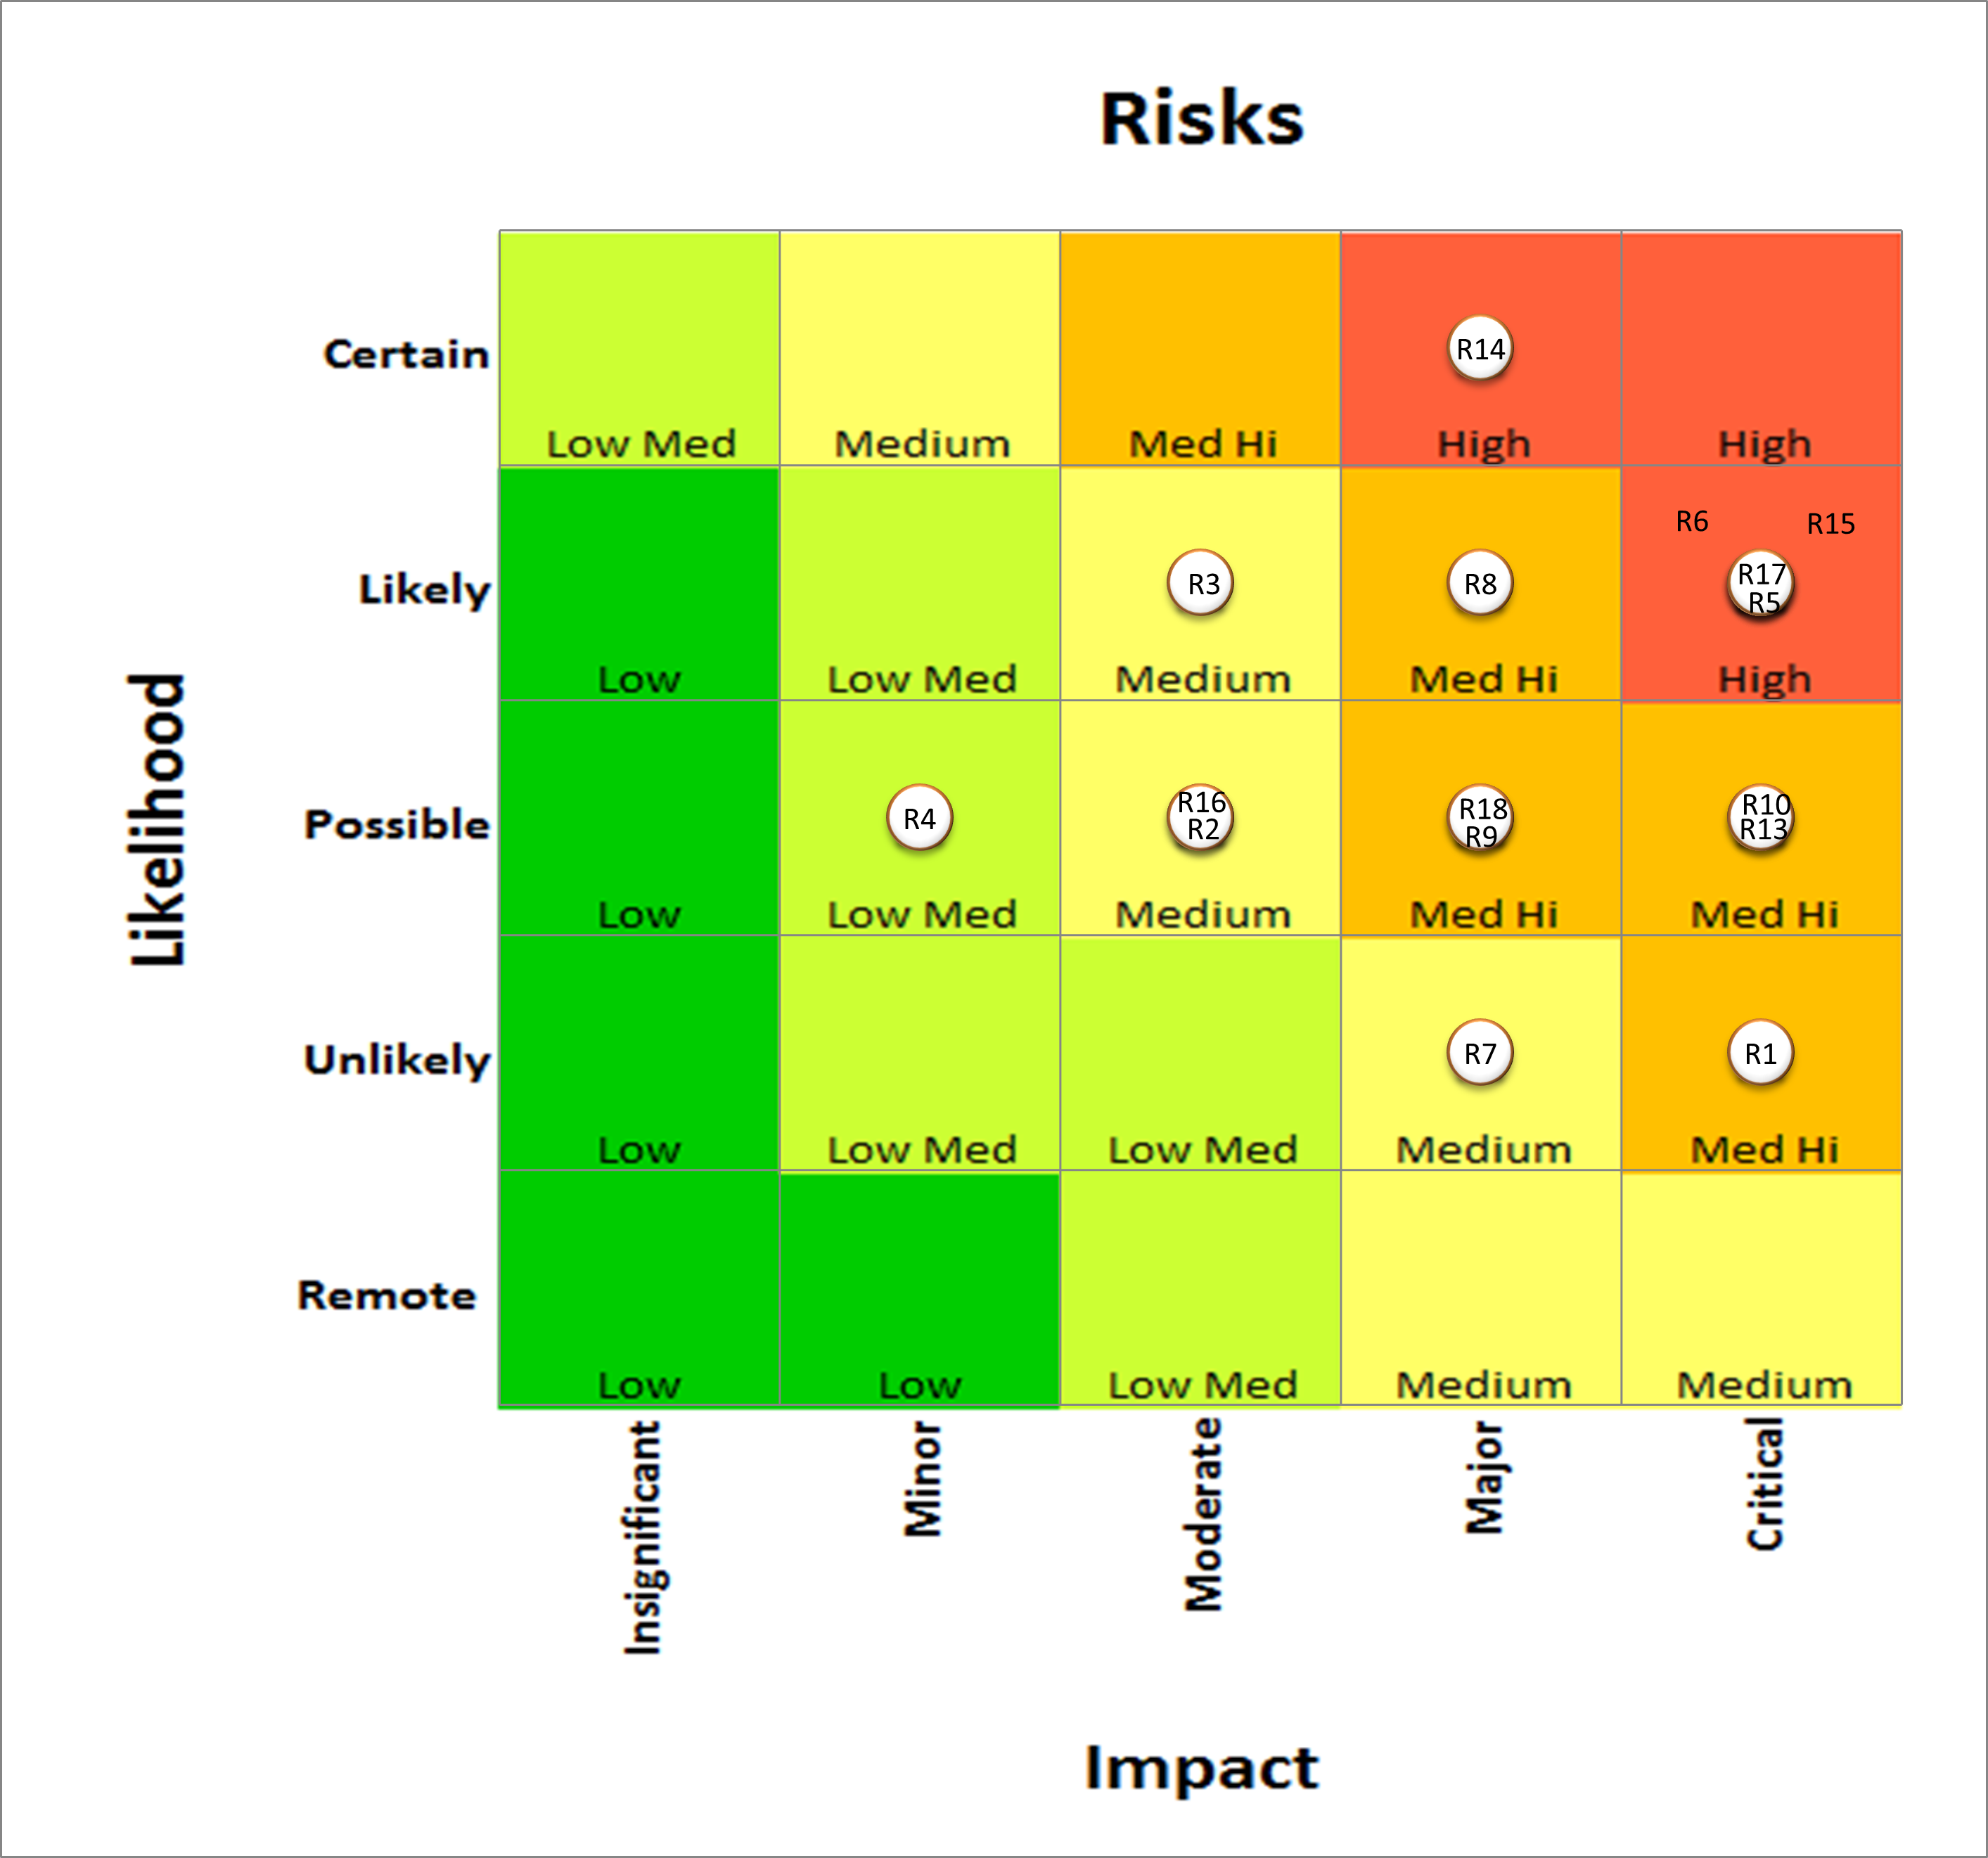
\includegraphics[width=1.0\textwidth]{img/risikomanagement/Risks.png}
  \caption{Risikomatrix}
  \label{fig:risk-matrix}
  \end{minipage} 
  \hfill
  \begin{minipage}[t]{0.45\linewidth}
  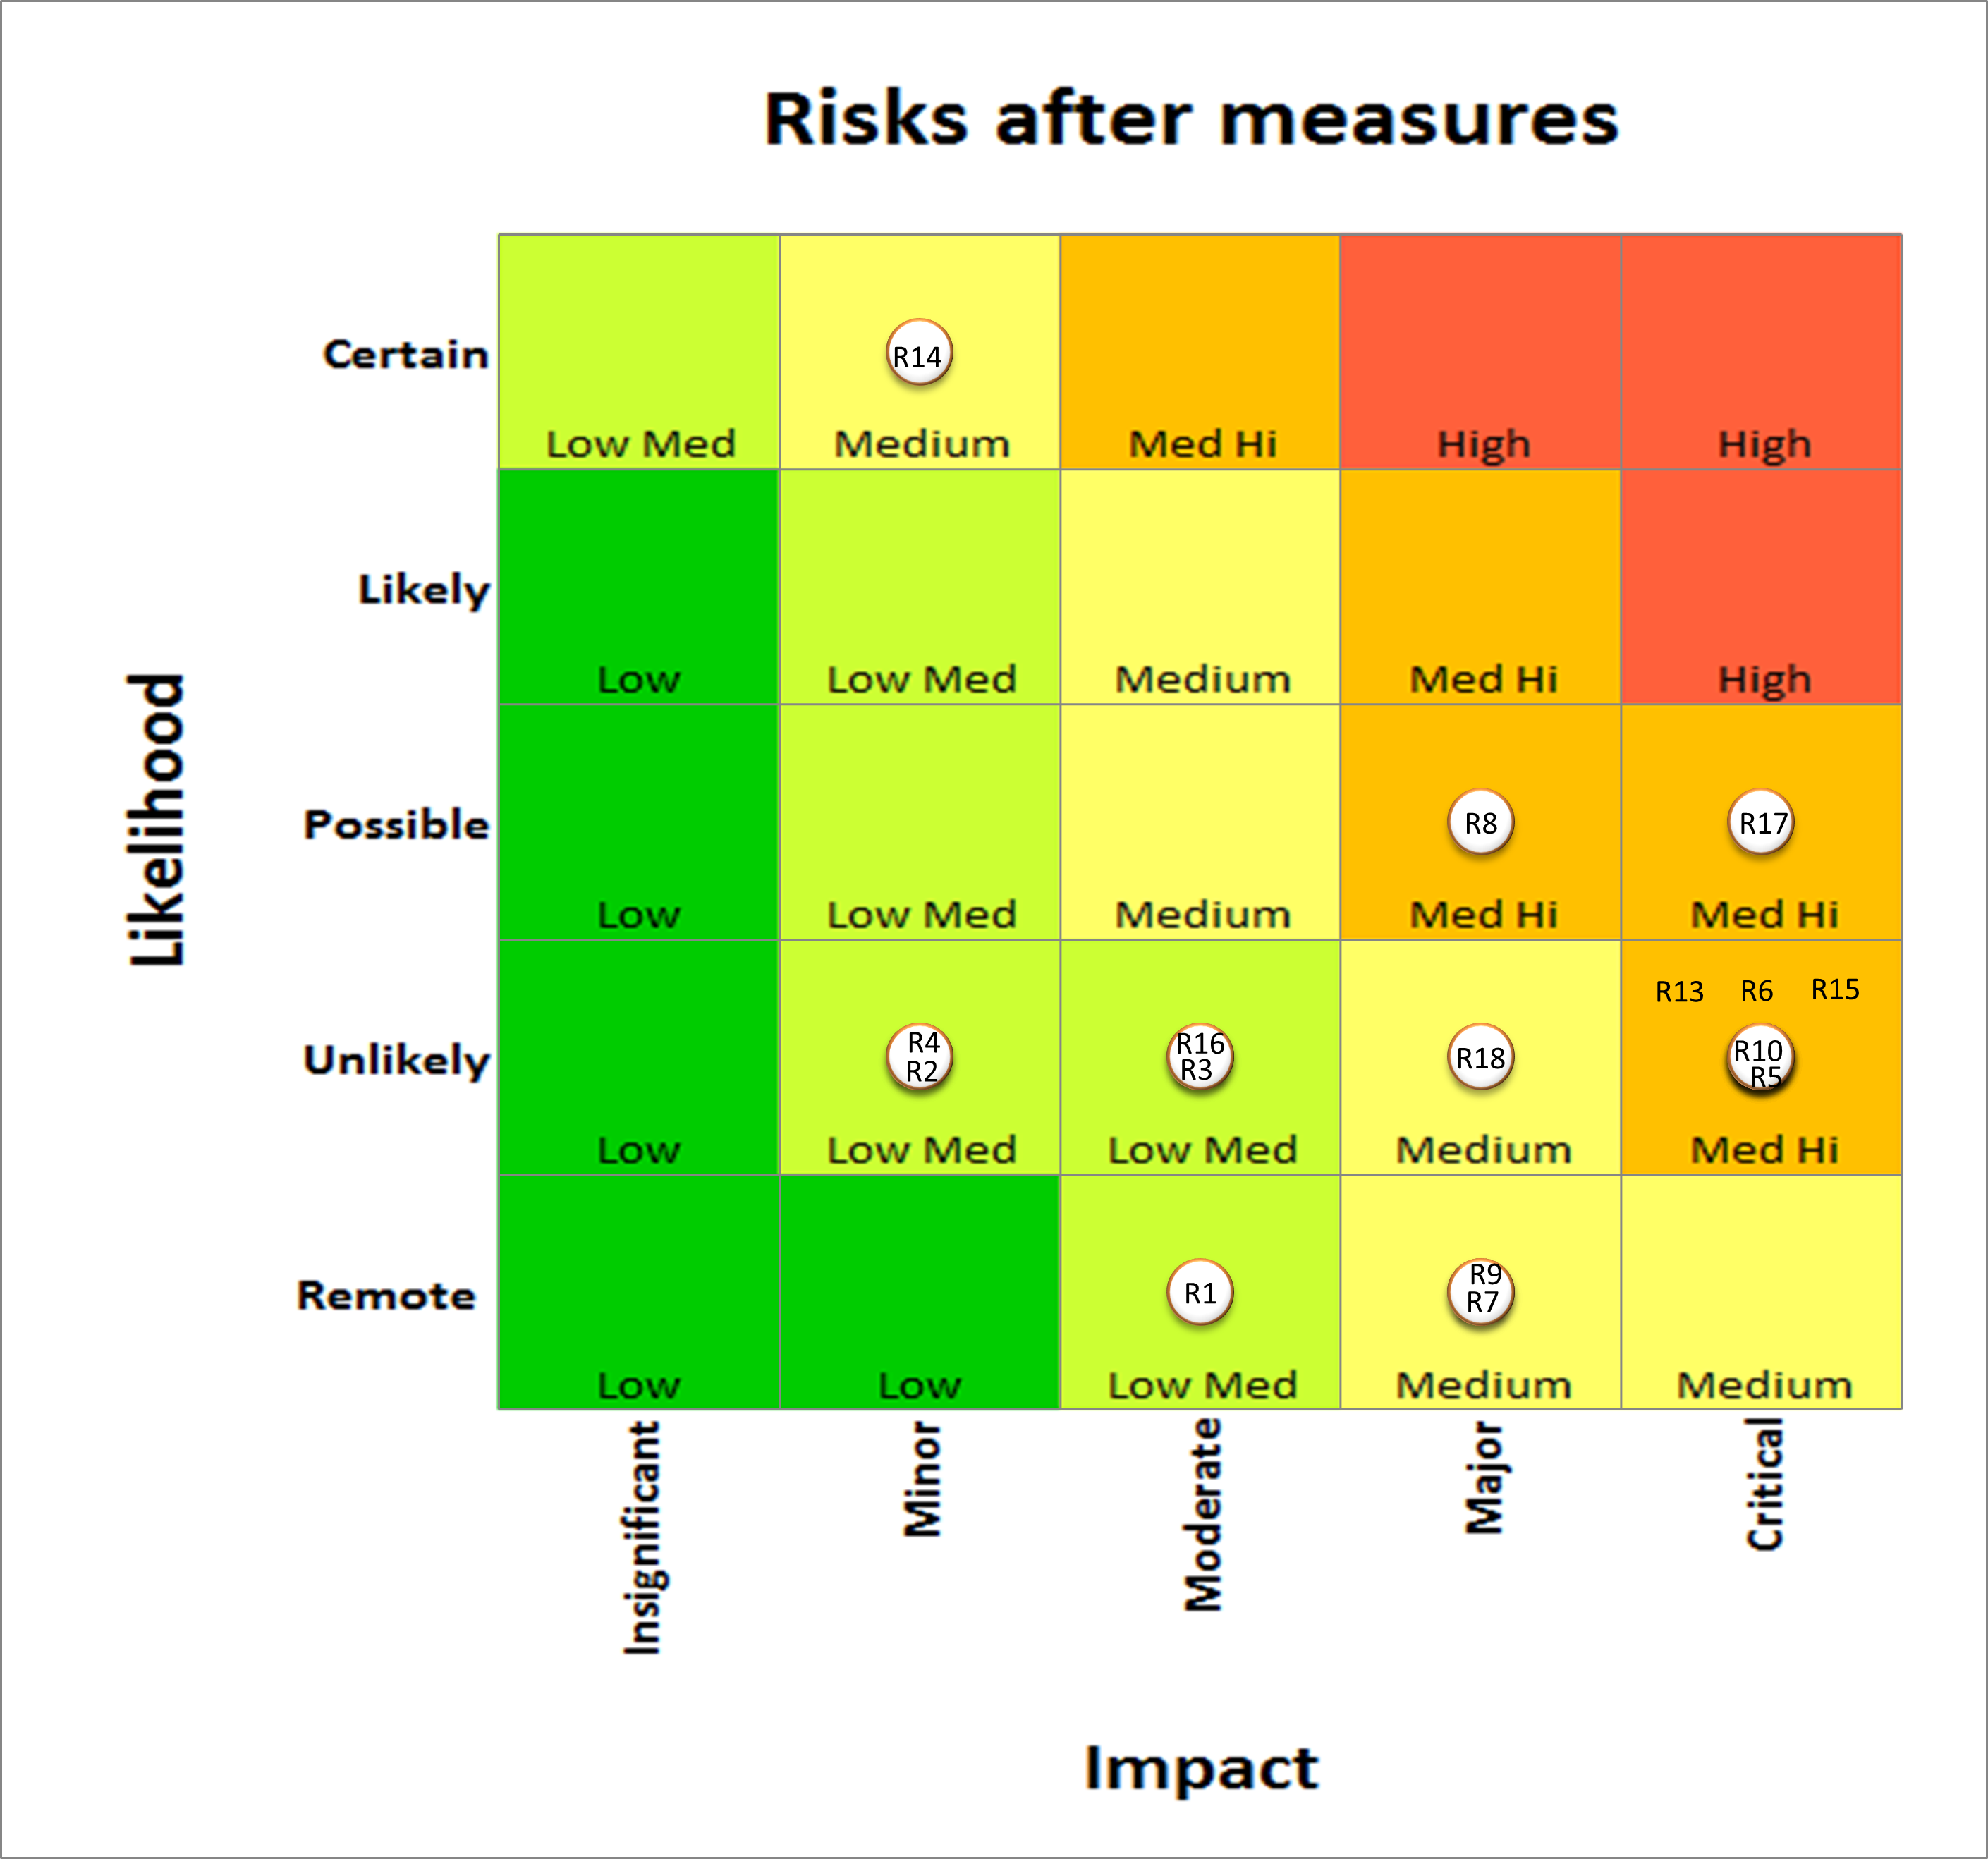
\includegraphics[width=1.0\textwidth]{img/risikomanagement/RisksAfterMeasures.png}
  \caption{Risikomatrix nach den präventiven Massnahmen}
  \label{fig:risk-matrix-after-measures}
  \end{minipage}
\end{figure}

\newpage
  
\subsection{Rahmenplan}
Wie in Abbildung \ref{fig:rahmenplan} ersichtlich, hat sich das Team dazu entschieden, dass Projekt in Sprints aufzuteilen. Diese dauern jeweils drei Wochen. Die drei Testate bilden die Meilensteine des Projekts im PREN 2.

\begin{figure}[H]
  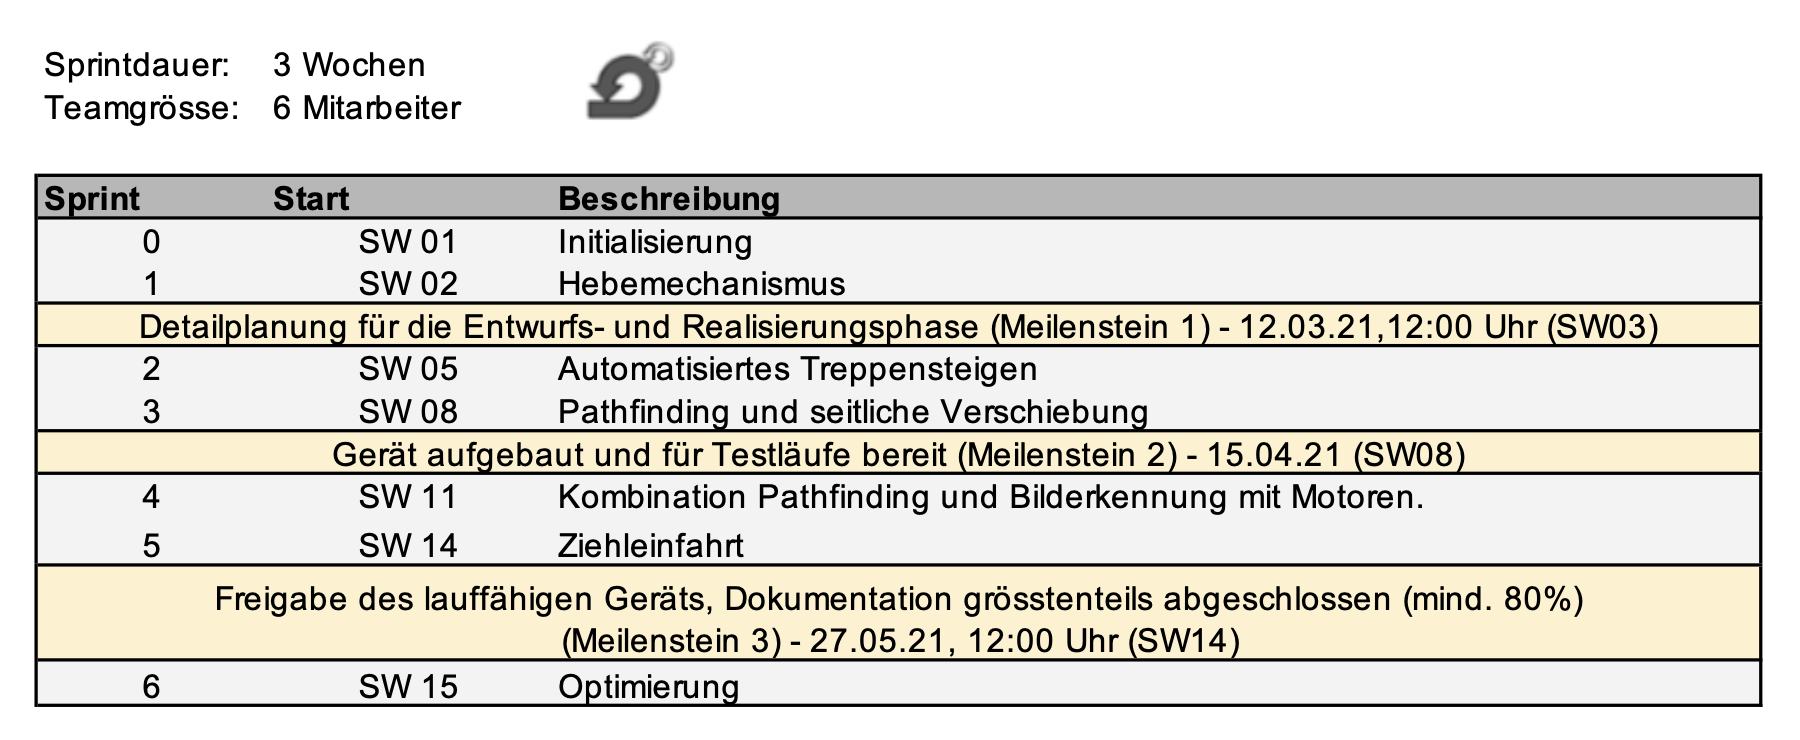
\includegraphics[width=1.0\textwidth]{img/projektmanagement/Rahmenplan PREN2.png}
  \centering
  \caption{Rahmenplan PREN 2}
  \label{fig:rahmenplan}
\end{figure}

\begin{figure}[H]
  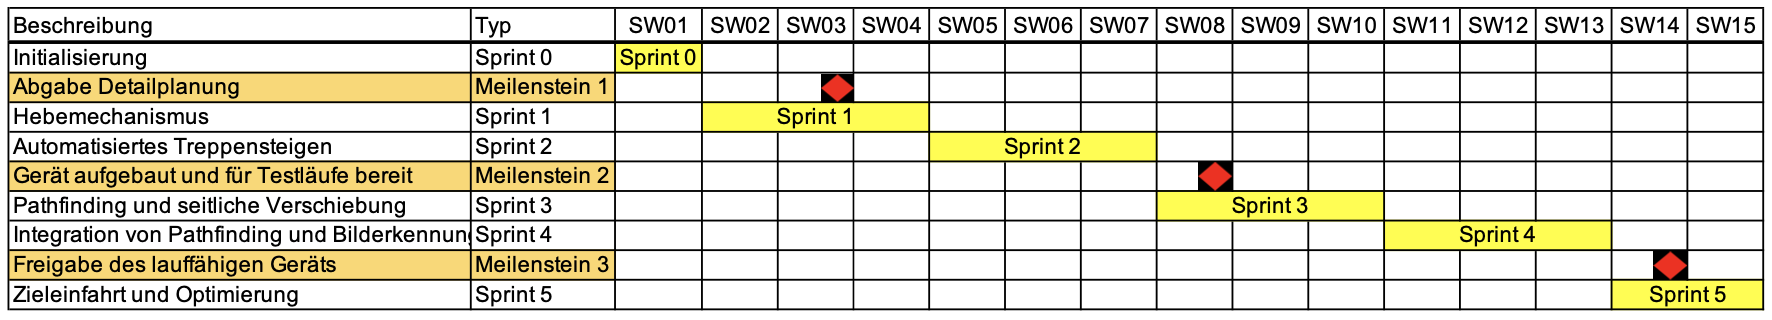
\includegraphics[width=1.0\textwidth]{img/projektmanagement/Zeitstrahl.png}
  \centering
  \caption{Zeitstrahl}
  \label{fig:sprint-backlog-1}
\end{figure}

\newpage

\subsection{Productbacklog}
Als zentrales Projektmanagement Element wird ein Productbacklog aufgesetzt. Dieser dient als Übersicht, was in den nächsten Sprints getan werden muss. Da für das \acrshort{pren2} Projekt jedoch ein klar vorgegebenen Zeitrahmen besteht, das Endresultat klar definiert und auch das Budget fixiert ist, werden bereits zu Beginn alle Sprints aufgelistet und grob geplant. 

Die Epics im Productbacklog und die daraus abgeleiteten User Storys im Sprintbacklog werden anhand von Storypoints eingeschätzt. Der Aufwand wird also nicht in Stunden abgeschätzt. Die Storypoints stehen auch nicht für eine gewisse Anzahl Stunden. Sie deuten lediglich darauf hin, dass der Aufwand für eine User Story mit 5 Story Points in etwa ein viertel so gross ist wie der Aufwand für eine Story mit 21 Story Points. Dies macht die Abschätzung deutlich einfacher, da es dem Menschen viel leichter fällt, den Aufwand relativ zu einem anderen Aufwand zu schätzen, als einen genauen Zeitaufwand anzugeben. Um die Sache noch ein wenig zu erleichtern, richten wir uns bei der Anzahl Story Points nach der Fibonacci-Reihe.

\begin{figure}[H]
  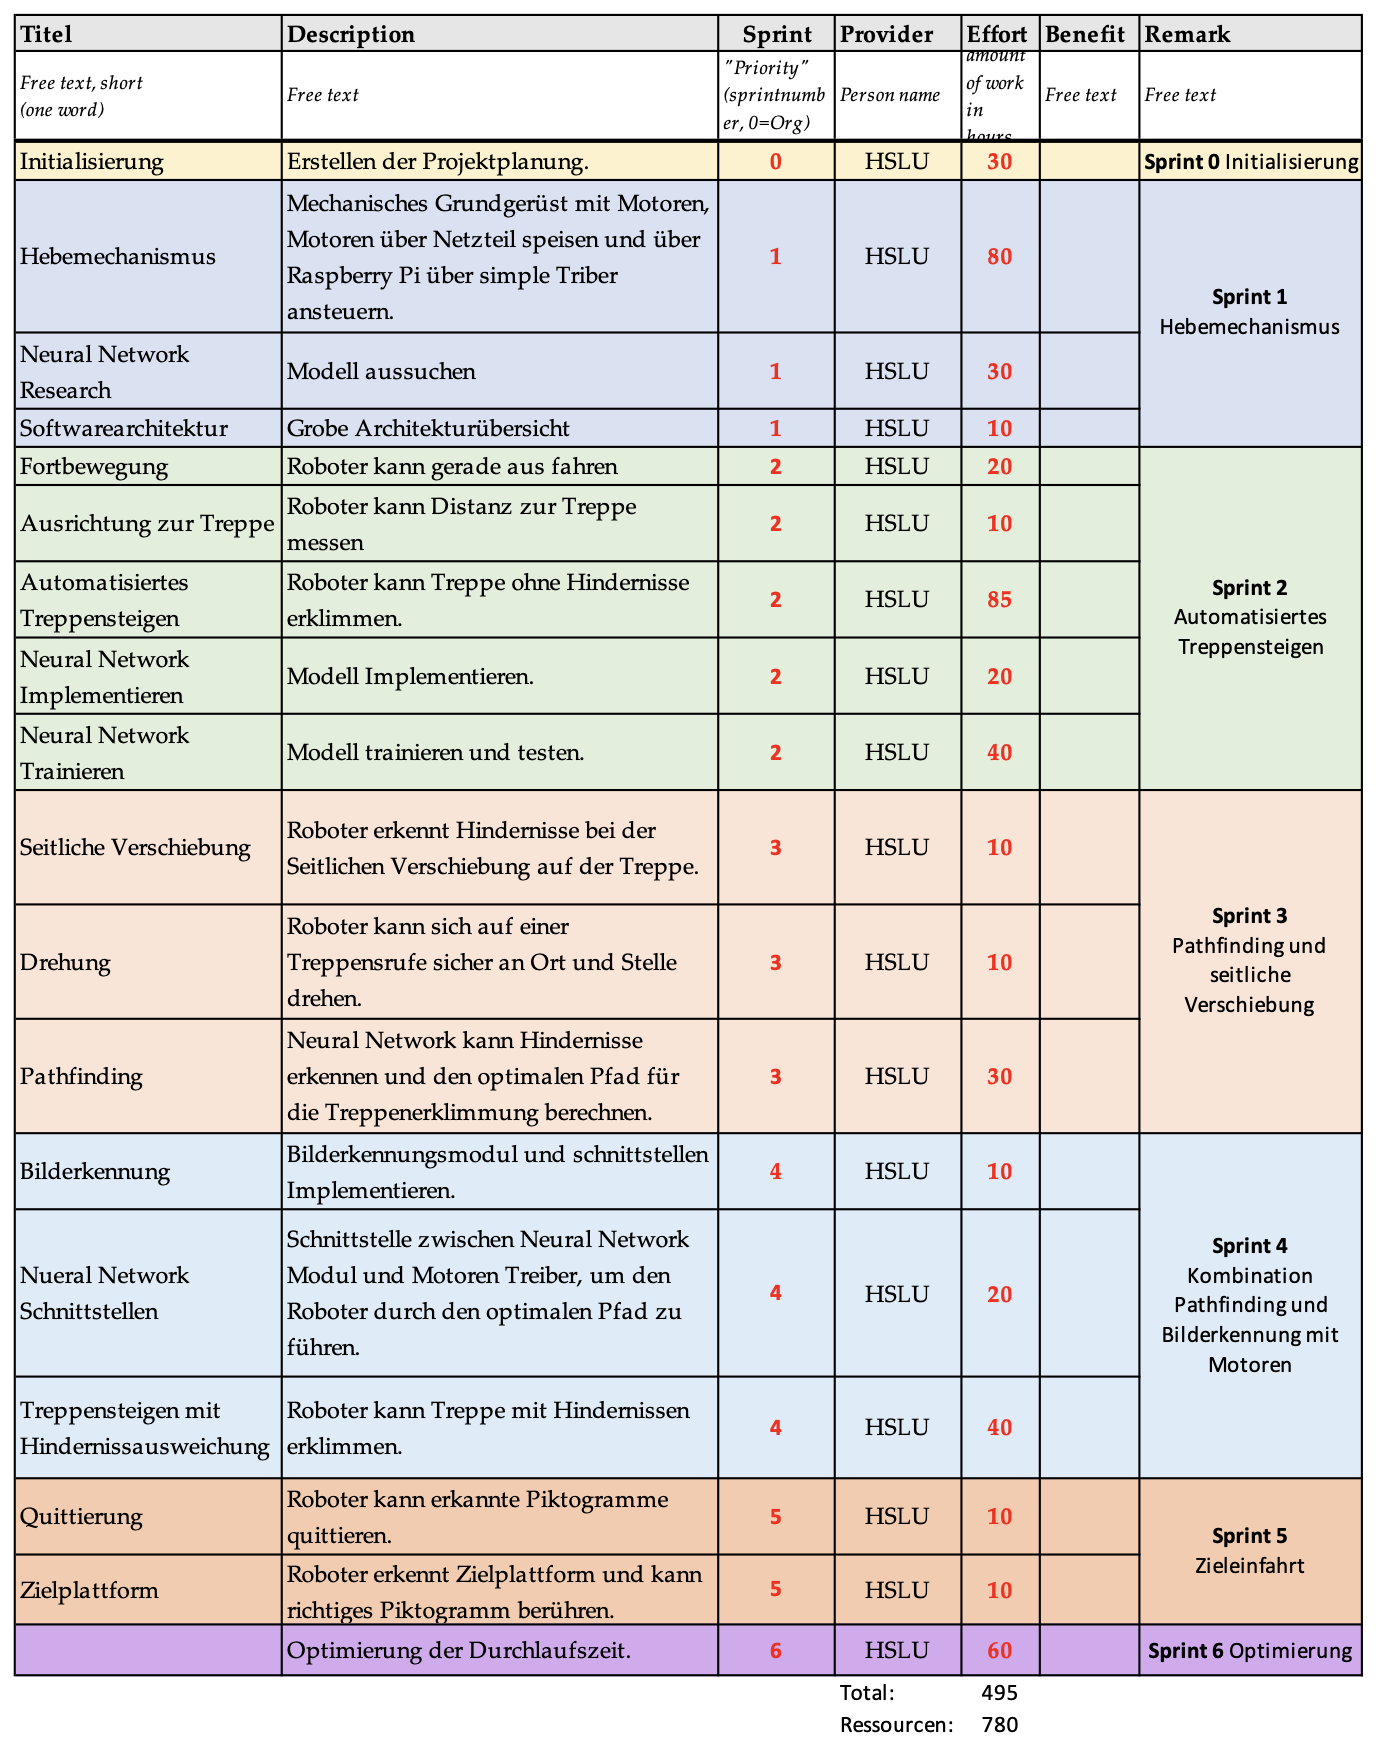
\includegraphics[width=0.95\textwidth]{img/projektmanagement/ProductBacklog PREN2.png}
  \centering
  \caption{Productbacklog}
  \label{fig:productbacklog}
\end{figure}


\subsection{Sprints}
Zu Beginn jedes Sprints wird eine Sprintplanung gemacht. Dazu werden die Backlog-Items (Epics) mit der höchsten Priorisierung in User-Storys aufgesplittet und in den Sprintbacklog übernommen. 

TODO: Boas Fibonacci Zahlen des Aufwands erklären

\subsubsection{Sprint 0}
\textbf{Sprintziel}\\
Das Ziel des nullten Sprints ist es, dass eine Detailplanung für die Entwurfs- und Realisierungsphase vorliegt. Zudem sollen die neuen Teammitglieder eingearbeitet sein und das Konzept aus Pren 1 verstehen. 

\textbf{Risiko-Update}\\
Es wurden die Top 3 Risiken welche am Ende von Pren 1 vorlagen übernommen: R1 (Drehung in der Nähe der Treppenwand), R2 (Gleichgewicht bei Erklimmung) und R3 (Roboter verschiebt Hindernisse).

\subsubsection{Sprint 1}
\textbf{Sprintziel}\\
Das Ziel von Sprint 1 ist es, dass mechanische Grundgerüst des Roboters zu erarbeiten. Dieses hat bereits die Motoren integriert und kann erfolgreich eine Hubbewegung tätigen. Weiter soll eine grobe Softwarearchitektur vorhanden sein.

\textbf{Risiko-Update}\\
Im Sprintplaning vom Sprint 1 sind die Risiken 4 (Technische Limitation Neural Network) und 5 (Unbekannte Position der Ausleger) hinzugekommen. 

\textbf{Sprintbacklog}\\
In der Abbildung \ref{fig:sprint-backlog-1} wird der Sprintbacklog gezeigt, welcher in der Sprintplanung erstellt wurde.
\begin{figure}[H]
  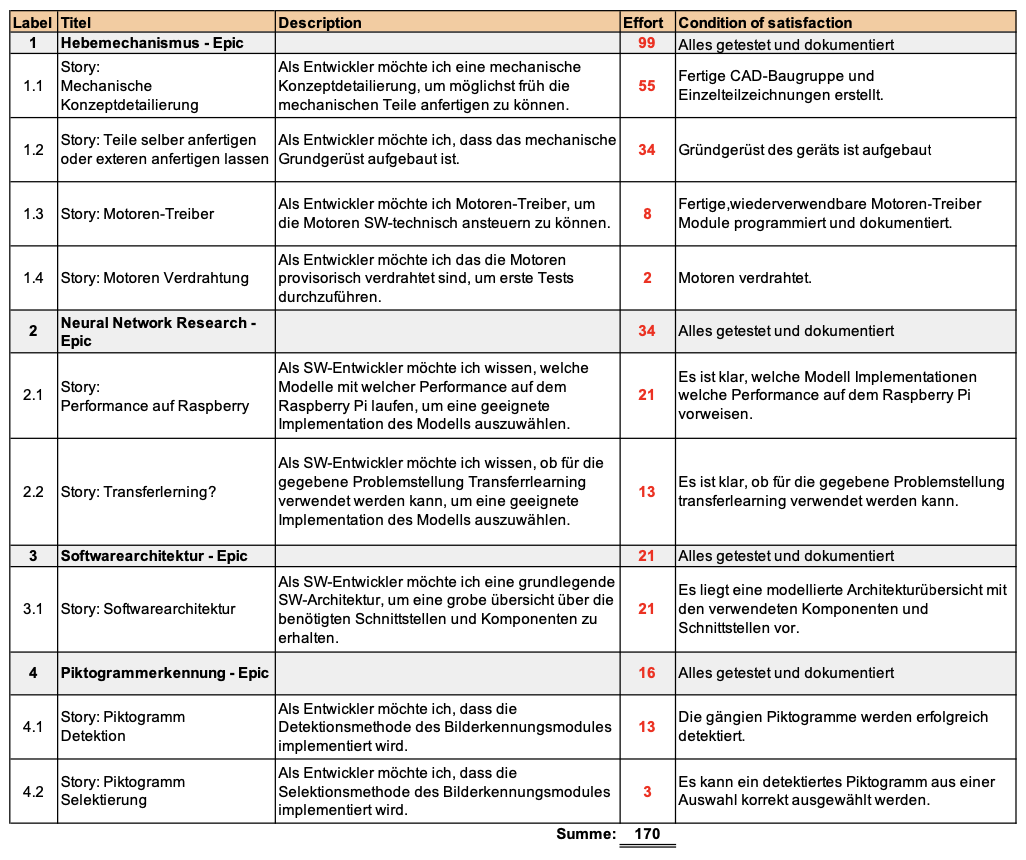
\includegraphics[width=1.0\textwidth]{img/projektmanagement/Sprint 1.png}
  \centering
  \caption{Sprint 1 - Backlog}
  \label{fig:sprint-backlog-1}
\end{figure}

\newpage

\textbf{Sprintreview}\\
Der erste Sprint konnte erfolgreich abgeschlossen werden. Im CAD wurde die Detailierung des Geräts fertig gestellt und von den Teilen, die extern gefertigt werden, wurden Einzelteilzeichnungen gemacht. Die Teile wurden in Auftrag gegeben. Weiter wurden diverse Teile selber 3D-gedruckt. Da im Team drei 3D-Drucker vorhanden sind, war es möglich vor Ende des ersten Sprints alle Teile anzufertigen. Die Teile, die in Auftrag gegeben wurden, wurden für den ersten Test der Hubbewegung auch mit dem 3D-Drucker hergestellt.
Die Elektrokomponenten wurden eingekauft und verdrahtet.
Der erste Test der Hubbewegungen war erfolgreich und hat die technische Machbarkeit des Konzepts bewiesen.

Das Teilziel Softwarearchitektur wurde ebenfalls erfolgreich abgeschlossen. Die Architektur wurde anhand einer FSM, einem Komponentendiagramm und UMLs dokumentiert. Der Grundriss der modellierte Architektur wurde in Python implementiert. Für jede Komponente wurde ein Feature-Branch vorbereitet. 
Weiter wurde aufgrund von Unterauslastung das Bilderkennungsepic von Sprint 4 in den Sprint 1 vorgeschoben. Die benötigten Module wurden implementiert, getestet und dokumentiert. 

\subsubsection{Sprint 2}
\textbf{Sprintziel}\\
Das Ziel von Sprint 2 ist es, die Treppe ohne Hindernisse geradeaus autonom erklimmen zu können. Dazu muss die Fartbewegung realisiert werden und das Gerätmuss sich vor einer Treppenstufe ausrichten können. Zudem soll das Pathfinding trainiert werden.

\textbf{Risiko-Update}\\
Das Risiko, dass die erste Hubbewegung technisch nicht umsetzbar ist, ist weggefallen, da der erste Test am Ende des ersten Sprints erfolgreich war.

\textbf{Sprintbacklog}\\
In der Abbildung \ref{fig:sprint-backlog-2} wird der Sprintbacklog gezeigt, welcher in der Sprintplanung erstellt wurde.
\begin{figure}[H]
  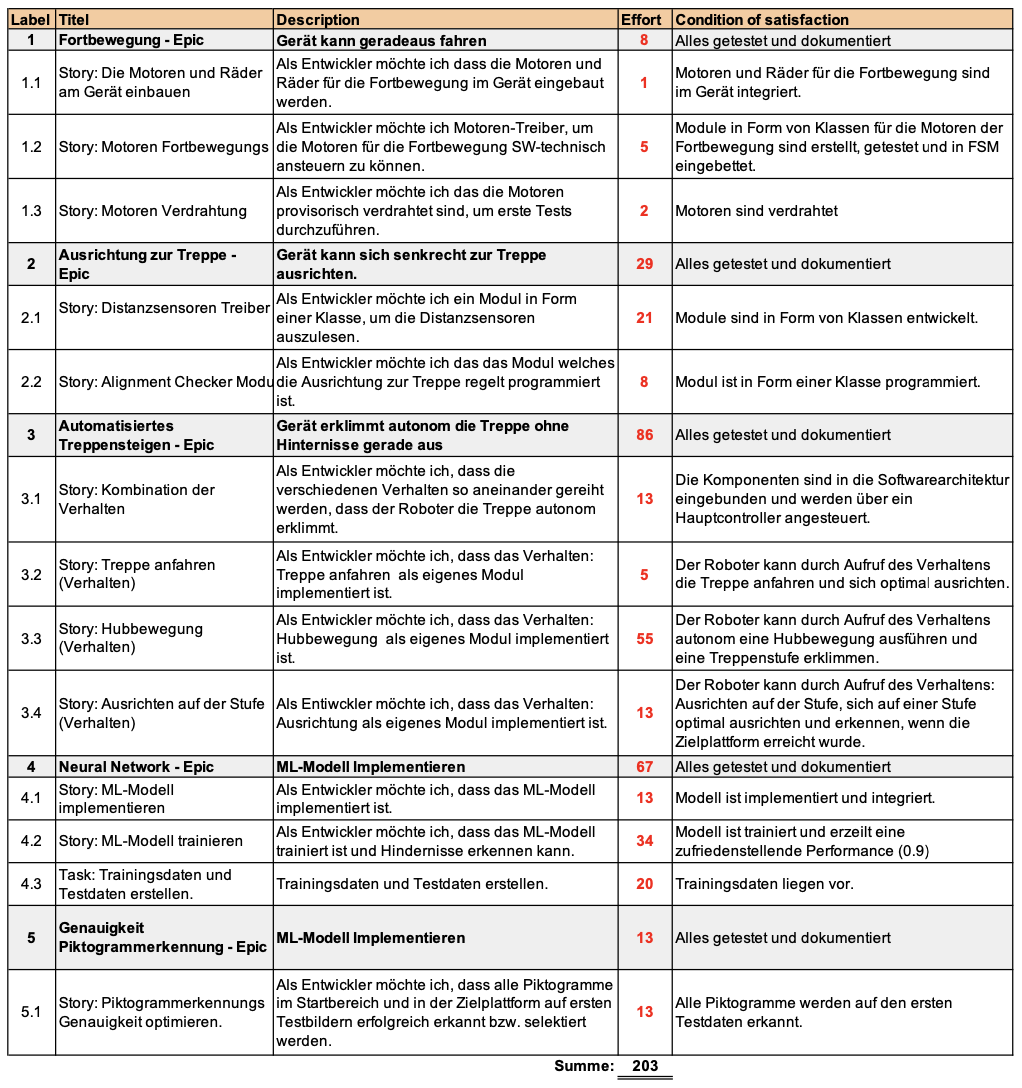
\includegraphics[width=1.0\textwidth]{img/projektmanagement/Sprint 2.png}
  \centering
  \caption{Sprint 2 - Backlog}
  \label{fig:sprint-backlog-2}
\end{figure}

\textbf{Sprintreview}\\
Die Fortbewegungskomponenten konnten im Gerät integriert werden und die Fortbewegung wurde erfolgreich manuell getestet. Auch die Ausrichtung vor einer Treppenstufe konnte umgesetzt werden. Das automatische Treppensteigen konnte noch nicht realisiert werden. Dieser Task wird im Sprint 3 weiter bearbeitet.


\subsubsection{Sprint 3}
\textbf{Sprintziel}\\
Im dritten Sprint soll die seitliche Verschiebung des Geräts auf einer Treppenstufe realisiert werden. Bei dieser Verschiebung sollen die Hindernisse mit mithilfe der Ultraschallsensoren erkannt werden. Weiter soll das automatisierte Treppensteigen realisiert werden, was bereits Ziel des zweiten Sprints war. Das Pathfinding soll so weit sein, dass der optimale Pfad für die Treppenbesteigung bestimmt werden kann.

\textbf{Risiko-Update}\\
Bezüglich der Fortbewegung wurden zwei neue Risiken erfasst, nämlich dass die Räder zu wenig Gripp haben und dass die Fortbewegungsmotoren zu wenig Drehmoment erzeugen.

\textbf{Sprintbacklog}\\
In der Abbildung \ref{fig:sprint-backlog-3} wird der Sprintbacklog gezeigt, welcher in der Sprintplanung erstellt wurde.
\begin{figure}[H]
  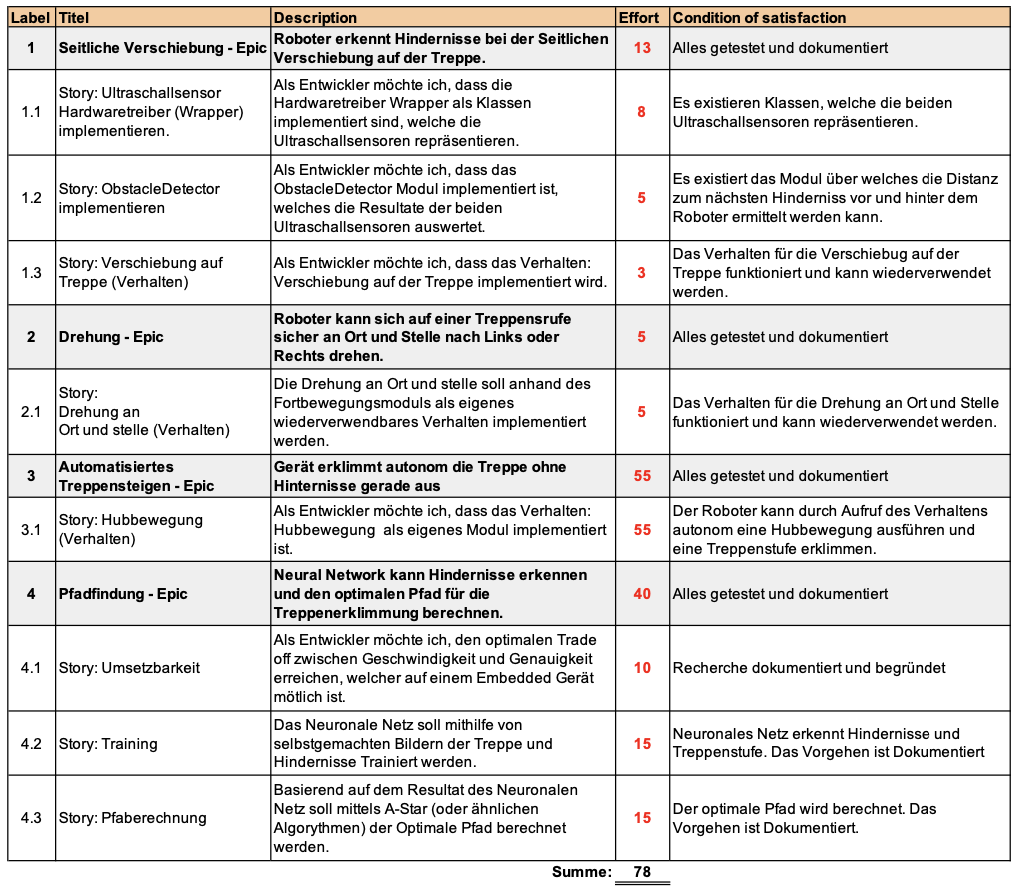
\includegraphics[width=1.0\textwidth]{img/projektmanagement/Sprint 3.png}
  \centering
  \caption{Sprint 3 - Backlog}
  \label{fig:sprint-backlog-3}
\end{figure}

\newpage

\textbf{Sprintreview}\\
Im Sprint 3 konnte der Wechsel von Raspberry Pi auf das Jetson Nano vorgenommen werden. Weiter wurde die sämtliche Verdrahtung aller elektronischen Komponenten vorgenommen. Das Verhalten für die 90° Drehung konnte implementiert werden, als auch eine Funktion welche eine bestimmte Distanz gerade aus fährt. Weiter wurden die Klassen welche die Ultraschallsensoren ansteuern implementiert und getestet. Die User Story 1.3: Seitliche Verscheibung (Verhalten) wurde noch nicht implementiert. Diese User Story wurde in Sprint 4 übernommen. Ebenfalls nicht erfüllt wurde die User Story 3.2: Kombination der Verhalten für automatisiertes Treppensteigen. Diese User Story wird ebenfalls in den Sprint 4 übernommen. Das Verhalten für eine einzelne Hubbewegung konnte jedoch soweit fertig gestellt und zeitlich bereits stark optimiert werden. Der Hauptgrund, weshalb das automatisierte Treppensteigen noch nicht funktioniert ist, dass der Wechsel vom Raspberry Pi auf das Jetson Nano unterschätzt wurde. Beim Wechsel gab es viele kleine Hürden. Eine der Hürden ist beispielsweise, dass das Jetson lediglich zwei PWM Signale generieren kann, obwohl drei benötigt werden.

\subsubsection{Sprint 4}
\textbf{Sprintziel}\\
Im vierten Sprint sollen die einzelnen Abläufe eines Laufes kombiniert werden. Das Gerät soll am Anfang ein Piktogramm erkennen und den optimalen Pfad auf der Treppe anhand der Hindernisserkennung berechnen um anschliessend die Treppe erfolgreich besteigen zu können. Zudem soll das Gerät fähig sein fünf verschiedene Piktogramme quittieren zu können. Das Gerät kann den ganzen Lauf, bis auf die Zieleinfahrt bewältigen.

\textbf{Risiko-Update}\\
Bezüglich dem Treppensteigen ist ein neues Risiko erkannt worden, nämlich dass das Gerät beim Erklimmen einer Stufe einen Schlag abbekommt, wenn das Gerät auf die Kante der nächsthöheren Stufe kippt.

\textbf{Sprintbacklog}\\
In der Abbildung \ref{fig:sprint-backlog-4} wird der Sprintbacklog gezeigt, welcher in der Sprintplanung erstellt wurde.
\begin{figure}[H]
  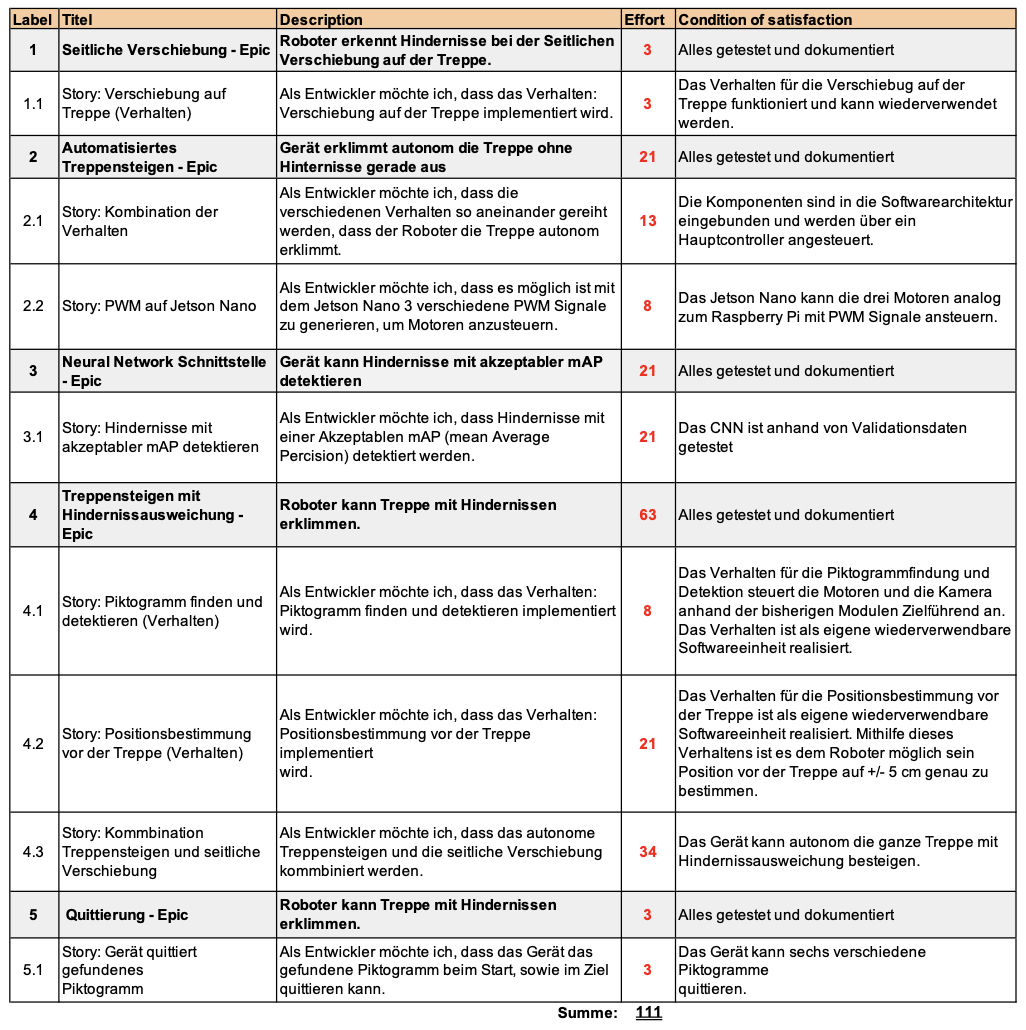
\includegraphics[width=1.0\textwidth]{img/projektmanagement/Sprint 4.png}
  \centering
  \caption{Sprint 4 - Backlog}
  \label{fig:sprint-backlog-4}
\end{figure}

\textbf{Sprintreview}\\
Der Sprint 4 war mehrheitlich erfolgreich. Die seitliche Verschiebung funktionert einwandfrei. Die zuerst als störend empfundenen Rillen der Treppe helfen dem Roboter beim traversieren sicher in der Spur zu bleiben. Weiter konnten verschiedene Module kombiniert werden. So wird das Piktogramm schnell gefunden und die Treppe direkt angefahren. Mithilfe der Pfadfindung wird der ideale Weg berechnet. Noch nicht getestet werden konnten die Distanzen zu den Hindernissen und die Positionierung vor der Treppe funktioniert noch nicht ideal. Dazu werden weitere Tests benötigt
Bei der Hardware wurde ein PWM  Board installiert welches über Hardware-PWM Pins verfügt. Dadurch können alle Motoren angesteuert werden und durch die Hardware PWMs laufen die Motoren verglichen zu den Software PWMs deutlich glatter.

\newpage

\subsubsection{Sprint 5}
\textbf{Sprintziel}\\
-

\textbf{Risiko-Update}\\
-

\textbf{Sprintbacklog}\\
-

\textbf{Sprintreview}\\

